\documentclass[a4paper,10pt]{article}

%% Packages
\usepackage{epigraph}
\usepackage{fancyhdr}
\usepackage{geometry}
\usepackage{hyperref}
\usepackage{setspace}
\usepackage{tabularx}

\usepackage[pdftex]{graphicx}
\usepackage{wrapfig}

%% Headers
\pagestyle{fancy}

\fancyhead[RO,RE]{\it Curriculum Vitae}
\fancyfoot[LO,LE]{\it Noortje J. Venhuizen, MSc}

\renewcommand{\headrulewidth}{0.2pt}
\renewcommand{\footrulewidth}{0.2pt}

%% Font
\usepackage{tgpagella}
\usepackage[T1]{fontenc}
\linespread{1.25}

%% Spacing
%\onehalfspacing

%% Right column width
\def\leftcolwidth{.15\textwidth}

%% Vertical spacing
\def\tablevspace{10pt}


\begin{document}

%%%%%%%%%%%%%%%%%%%%%%%%%%%%%%%%%%%%%%%%%%%%%%%%%%%%%%%%%%%%%%%%%%%%%%%%%%
%% Name                                                                 %%
%%%%%%%%%%%%%%%%%%%%%%%%%%%%%%%%%%%%%%%%%%%%%%%%%%%%%%%%%%%%%%%%%%%%%%%%%%

\begin{flushright}
{\Huge Noortje J. Venhuizen, MSc}
\end{flushright}

%%%%%%%%%%%%%%%%%%%%%%%%%%%%%%%%%%%%%%%%%%%%%%%%%%%%%%%%%%%%%%%%%%%%%%%%%%
%% Personal Information                                                 %%
%%%%%%%%%%%%%%%%%%%%%%%%%%%%%%%%%%%%%%%%%%%%%%%%%%%%%%%%%%%%%%%%%%%%%%%%%%

\section*{Personal Information}

\begin{wrapfigure}{r}{0.5\textwidth}
  \begin{flushright}
  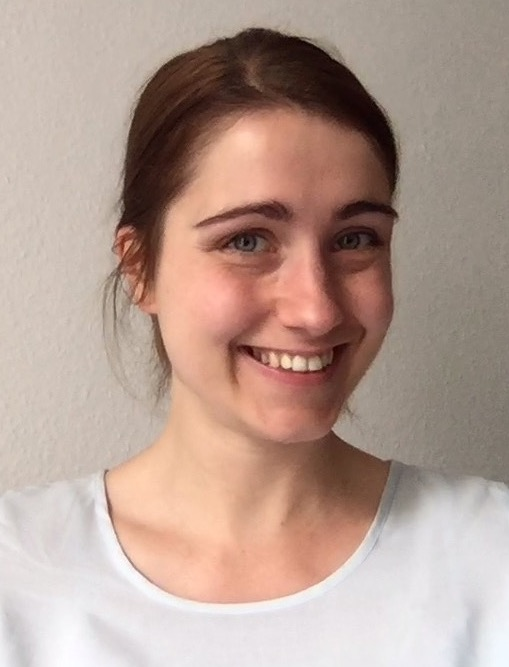
\includegraphics[width=0.3\textwidth]{noortje.jpg}
  \end{flushright}
\end{wrapfigure}

%% Name
\noindent
\begin{tabularx}{\textwidth}{ p{\leftcolwidth} X }
  Full name:      &         Noortje Joost Venhuizen\\
\end{tabularx}

\vspace{\tablevspace}

%% Birth and Nationality
\noindent
\begin{tabularx}{\textwidth}{ p{\leftcolwidth} X }
  Date of birth:  &         19--10--1986 (October 19th, 1986)\\
  Birthplace:     &         Groningen, The Netherlands\\
  Nationality:    &         Dutch\\
  BSN:            &         199354261\\
\end{tabularx}

\vspace{\tablevspace}

%% E-mail address
\noindent
\begin{tabularx}{\textwidth}{ p{\leftcolwidth} X }
  E-mail:         &         \href{mailto:n.j.venhuizen@rug.nl}{n.j.venhuizen@rug.nl}\\
\end{tabularx}

\vspace{\tablevspace}

%% Personal homepage
\noindent
\begin{tabularx}{\textwidth}{ p{\leftcolwidth} X }
  Homepage:       &       \url{http://www.let.rug.nl/venhuizen/}\\
                  &       \url{http://noortjejoost.github.io}
\end{tabularx}


%%%%%%%%%%%%%%%%%%%%%%%%%%%%%%%%%%%%%%%%%%%%%%%%%%%%%%%%%%%%%%%%%%%%%%%%%%
%% Education                                                            %%
%%%%%%%%%%%%%%%%%%%%%%%%%%%%%%%%%%%%%%%%%%%%%%%%%%%%%%%%%%%%%%%%%%%%%%%%%%

\section*{Education}

\noindent
\begin{tabularx}{\textwidth}{ p{\leftcolwidth} X }
  2011 -- 2015
  & \textbf{PhD degree in Computational Semantics}\\
  & `Robust Presupposition Projection'\\
  & \textit{Center for Language and Cognition Groningen (CLCG)}\\
  & \textit{University of Groningen}\\
  & \\
  & Promotores: Prof. dr. J. Bos and Prof. dr. P. Hendriks
\end{tabularx}

\vspace{\tablevspace}

%% MSc in Logic
\noindent
\begin{tabularx}{\textwidth}{ p{\leftcolwidth} X }
  2009 -- 2011  
  & \textbf{MSc degree in Logic}\\
  & Track: `Logic \& Language'\\
  & \textit{Institute for Logic, Language and Computation (ILLC)}\\
  & \textit{University of Amsterdam}\\
  & \\
  & Thesis: `Negation in Questions'\\
  & Advisors: dr. F. Roelofsen and dr. G. Weidman Sassoon\\
\end{tabularx}

\vspace{\tablevspace}

%% BA in Artificial Intelligence
\noindent
\begin{tabularx}{\textwidth}{ p{\leftcolwidth} X }
  2006 -- 2009  
  & \textbf{BA degree in Artificial Intelligence} (\textit{cum laude})\\
  & \textit{University of Utrecht}\\
  & \\
  & Thesis: `Donkey anaphora and Skolem functions'\\
  & Advisor: dr. Y. Winter\\
\end{tabularx}

\vspace{\tablevspace}

%% Other relevant training

\subsection*{Other relevant training}

\noindent
\begin{tabularx}{\textwidth}{ p{\leftcolwidth} X }
  2013 & \textbf{LOT Summer School 2013}, June 17-28 \textit{(Certificate acquired)}\\
       & \textit{Groningen, the Netherlands}\\
       & -- {Masterclass Semantics and Pragmatics} (Prof. dr. L.B.W. Geurts)\\
       & -- {Quantity Implicatures} (Prof. dr. L.B.W. Geurts)\\
       & -- {Neurobiology of Language -- State of the Art} (dr. J.C.J. Hoeks)\\
       & \\
  2012 & \textbf{LOT Summer School 2012}, July 2-13 \textit{(Certificate acquired)}\\
       & \textit{Utrecht, the Netherlands}\\
       & -- {Masterclass Discourse Interpretation} (Prof. dr. A. Kehler)\\
       & -- {Reference and Coherence in Discourse} (Prof. dr. A. Kehler)\\
       & -- {Discourse and Cognition -- State of the Art} (Prof. dr. T.J.M. Sanders)\\
       & -- {Implicit Learning and Second Language Acquisition}
         (dr. P. Rebuschat)\\
       & \\
  2005 & \textbf{Curso de Lingua Portuguesa para Estrangeiros} 
         \textit{(Certificate acquired)}\\
       & \textit{Universidade de Coimbra, Portugal}\\
       & ``Portuguese as a foreign language'' (Annual course)\\

\end{tabularx}

%%%%%%%%%%%%%%%%%%%%%%%%%%%%%%%%%%%%%%%%%%%%%%%%%%%%%%%%%%%%%%%%%%%%%%%%%%
%% Work Experience                                                      %%
%%%%%%%%%%%%%%%%%%%%%%%%%%%%%%%%%%%%%%%%%%%%%%%%%%%%%%%%%%%%%%%%%%%%%%%%%%

%\section*{Work Experience}

%%%%%%%%%%%%%%%%%%%%%%%%%%%%%%%%%%%%%%%%%%%%%%%%%%%%%%%%%%%%%%%%%%%%%%%%%%
%% Teaching Experience                                                  %%
%%%%%%%%%%%%%%%%%%%%%%%%%%%%%%%%%%%%%%%%%%%%%%%%%%%%%%%%%%%%%%%%%%%%%%%%%%

\section*{Teaching Experience}

%% Guest Lecture
\noindent
\begin{tabularx}{\textwidth}{ p{\leftcolwidth} X }
  2014
  & \textbf{Guest Lecturer: Linguistic Theory---Semantics}\\
  & Talk: `Discourse Representation Theory and its applications'\\
  & Teacher: Prof. dr. P. Hendriks\\
  & \textit{Research Master Linguistics, University of Groningen}\\
\end{tabularx}

\vspace{\tablevspace}

%% Guest Lecture
\noindent
\begin{tabularx}{\textwidth}{ p{\leftcolwidth} X }
  2013
  & \textbf{Guest Lecturer: Syntactic and Semantic Theory}\\
  & Talk: `Introducing DRT and PDRT'\\
  & Teacher: Prof. dr. P. Hendriks\\
  & \textit{Research Master Linguistics, University of Groningen}\\
\end{tabularx}

\vspace{\tablevspace}

%% Textmanipulatie
\noindent
\begin{tabularx}{\textwidth}{ p{\leftcolwidth} X }
  2013
  & \textbf{Teacher: Textmanipulatie (UNIX tools)}\\
  & \textit{Bachelor Information Science, University of Groningen}\\
\end{tabularx}

\vspace{\tablevspace}

\noindent
\begin{tabularx}{\textwidth}{ p{\leftcolwidth} X }
  2012
  & \textbf{Teacher: Textmanipulatie (UNIX tools)}\\
  & \textit{Bachelor Information Science, University of Groningen}\\
\end{tabularx}

\vspace{\tablevspace}

%% TA Logic
\noindent
\begin{tabularx}{\textwidth}{ p{\leftcolwidth} X }
  2010, 2011
  & \textbf{Teaching assistant: Logic}\\
  & Teacher: dr. J. Jaspars\\
  & \textit{Bachelor Beta-Gamma, University of Amsterdam}\\
\end{tabularx}

\vspace{\tablevspace}

%% TA Mathematical Logic
\noindent
\begin{tabularx}{\textwidth}{ p{\leftcolwidth} X }
  2010
  & \textbf{Teaching assistant: Introduction to Mathematical Logic}\\
  & Teacher: Prof.dr. Y. Venema\\
  & \textit{Bachelor Mathematics, University of Amsterdam}\\
\end{tabularx}

%%%%%%%%%%%%%%%%%%%%%%%%%%%%%%%%%%%%%%%%%%%%%%%%%%%%%%%%%%%%%%%%%%%%%%%%%%
%% Other Activities                                                     %%
%%%%%%%%%%%%%%%%%%%%%%%%%%%%%%%%%%%%%%%%%%%%%%%%%%%%%%%%%%%%%%%%%%%%%%%%%%

\section*{Other Activities}

%% Reviewer for: Proceeedings of *SEM 2012; TABU dag 2013; *SEM 2013, ...

%% Local organisation LOT summer school 2013
\noindent
\begin{tabularx}{\textwidth}{ p{\leftcolwidth} X }
  2013
  & \textbf{Member Local organisation LOT Summer School 2013}\\
  & \textit{CLCG, University of Groningen}\\
\end{tabularx}

\vspace{\tablevspace}

%%Studentlid Faculteitsraad Geesteswetenschappen
\noindent
\begin{tabularx}{\textwidth}{ p{\leftcolwidth} X }
  2009-2010
  & \textbf{Member Student's Council (Student-lid Faculteitsraad)}\\
  & \textit{Faculty of Humanities, University of Utrecht}\\
\end{tabularx}

\vspace{\tablevspace}

%% Surveilleren
%\noindent
%\begin{tabularx}{\textwidth}{ p{\leftcolwidth} X }
%  2008-2009
%  & \textbf{Exam invigilator}\\
%  & \textit{BV Topselect detacheringen, Utrecht}\\
%\end{tabularx}

\vspace{\tablevspace}

%% Huiswerkassistent
\noindent
\begin{tabularx}{\textwidth}{ p{\leftcolwidth} X }
  2007-2009
  & \textbf{Tutor/ homework assistant}\\
  & Subjects: Mathematics, Physics\\
  & \textit{StudentsPlus, Utrecht}
\end{tabularx}

\vspace{\tablevspace}

%% OC lid
\noindent
\begin{tabularx}{\textwidth}{ p{\leftcolwidth} X }
  2007-2008
  & \textbf{Student member Education Committee (OC)}\\
  & \textit{Bachelor Artificial Intelligence, University of Utrecht}\\
\end{tabularx}

%\vspace{\tablevspace}

%%%%%%%%%%%%%%%%%%%%%%%%%%%%%%%%%%%%%%%%%%%%%%%%%%%%%%%%%%%%%%%%%%%%%%%%%%
%% Publications                                                         %%
%%%%%%%%%%%%%%%%%%%%%%%%%%%%%%%%%%%%%%%%%%%%%%%%%%%%%%%%%%%%%%%%%%%%%%%%%%

\section*{Publications}

%% In Preparation
%\subsection*{In Preparation}

%%Accepted 
\subsection*{Conference Proceedings}

\noindent
\begin{tabularx}{\textwidth}{ X }

    \textbf{Venhuizen, N.J.}, Bos, J., Hendriks, P., and Brouwer, H. (2014):
    How and Why Conventional Implicatures Project. In Todd Snider et al.
    (eds.), \textit{Proceedings of Semantics and Linguistic Theory (SALT) 24},
    63-83, New York, USA.\\
    \\
    \textbf{Venhuizen, N. J.} and Brouwer, H. (2014): PDRT-SANDBOX: An implementation
    of Projective Discourse Representation Theory. In Verena Rieser and
    Philippe Muller (eds.), \textit{Proceedings of the 18th Workshop on the
    Semantics and Pragmatics of Dialogue (SemDial-DialWatt 2014)}, 249-251,
    September 1-3, Edinburgh, Scotland.\\
    \\
    \textbf{Venhuizen, N.J.}, Bos, J. and Brouwer, H. (2013): Parsimonious 
    Semantic Representations with Projection Pointers. In \textit{Proceedings
    of the 10th International Conference on Computational Semantics (IWCS 2013)
    -- Long papers}, Potsdam, Germany.\\
    \\
    \textbf{Venhuizen, N.J.}, Basile, V., Evang, K. and Bos, J. (2013):
    Gamification for Word Sense Labeling. In \textit{Proceedings of the 10th 
    International Conference on Computational Semantics (IWCS 2013) --
    Short papers}, Potsdam, Germany.\\
    \\
    Roelofsen, F., \textbf{Venhuizen, N.J.} and Weidman Sassoon, G. (2013):
    Positive and negative polar questions in discourse. In \textit{Proceedings of
    Sinn und Bedeutung} 17, Paris, France.\\
    \\
    Basile, V., Bos, J., Evang, K. and \textbf{Venhuizen, N.J.} (2012): UGroningen:
    Negation detection with Discourse Representation Structures. In
    \textit{Proceedings of the First Joint Conference on Lexical and Computational
    Semantics (*SEM'12)}, Montr\'eal, Canada.\\
    \\
    Basile, V., Bos, J., Evang, K. and \textbf{Venhuizen, N.J.} (2012): Developing
    a large semantically annotated corpus. In \textit{Proceedings of the 8th
    International Conference on Language Resources and Evaluation (LREC'12)},
    Istanbul, Turkey.\\
    \\
    Basile, V., Bos, J., Evang, K. and \textbf{Venhuizen, N.J.} (2012): A platform
    for collaborative semantic annotation. In \textit{Proceedings of the
    Demonstrations at the 13th Conference of the European Chapter of the
    Association for Computational Linguistics (EACL'12)}, Avignon, France.\\
\end{tabularx}

%% Talks
\subsection*{Talks}

\noindent
\begin{tabularx}{\textwidth}{ X }
    \textbf{Venhuizen, N. J.} and Brouwer, H. (2014): Harnessing Projection: A Formal
    Implementation of Projective Discourse Representation Theory. Talk
    presented at the 24rd Meeting of Computational Linguistics in the
    Netherlands (CLIN 2014), January 17, Leiden, The Netherlands.\\
    \\
    \textbf{Venhuizen, N.J.} (2013): Factive presuppositions in discourse:
    Towards a formal analysis in PDRT. Talk presented at the 34th TABU Dag,
    June 13-14, Groningen, the Netherlands.\\
    \\
    \textbf{Venhuizen, N.J.}, Bos, J. and Brouwer, H. (2013): Parsimonious 
    Semantic Representations with Projection Pointers. Talk presented at the
    Computational Linguistics Reading Group, University of Groningen, March 15,
    Groningen, the Netherlands.\\
    \\
    \textbf{Venhuizen, N.J.} (2012): Projection Phenomena in Discourse. Talk
    presented in the masterclass on Discourse Interpretation, LOT Summer
    School 2012, July 4, Utrecht, the Netherlands.\\
    \\
    \textbf{Venhuizen, N.J.} (2012): Representing Projection Phenomena in DRT. Talk
    presented at the 22nd Meeting of Computational Linguistics in the
    Netherlands (CLIN 2012), January 20th, Tilburg, the Netherlands.\\
\end{tabularx}

%% Posters
\subsection*{Posters}

\noindent
\begin{tabularx}{\textwidth}{ X }
    Basile, V., Bos, J., Evang, K. and \textbf{Venhuizen, N.J.} (2013): Wordrobe: 
    using Games with a Purpose for Linguistic Annotation. Poster presented at 
    the 23rd Meeting of Computational Linguistics in the Netherlands 
    (CLIN 2013), January 18, Enschede, the Netherlands.\\
    \\
    Basile, V., Bos, J., Evang, K. and \textbf{Venhuizen, N.J.} (2012): Creating
    a semantically annotated corpus based on Discourse Representation
    Theory. Poster presented at the 22nd Meeting of Computational
    Linguistics in the Netherlands (CLIN 2012), January 20, Tilburg, 
    the Netherlands.\\
\end{tabularx}


%%%%%%%%%%%%%%%%%%%%%%%%%%%%%%%%%%%%%%%%%%%%%%%%%%%%%%%%%%%%%%%%%%%%%%%%%%
%% Grants                                                               %%
%%%%%%%%%%%%%%%%%%%%%%%%%%%%%%%%%%%%%%%%%%%%%%%%%%%%%%%%%%%%%%%%%%%%%%%%%%

%%helaas...

%%%%%%%%%%%%%%%%%%%%%%%%%%%%%%%%%%%%%%%%%%%%%%%%%%%%%%%%%%%%%%%%%%%%%%%%%%
%% Honors and Awards                                                    %%
%%%%%%%%%%%%%%%%%%%%%%%%%%%%%%%%%%%%%%%%%%%%%%%%%%%%%%%%%%%%%%%%%%%%%%%%%%

\section*{Honors and Awards}

\noindent
\begin{tabularx}{\textwidth}{ p{\leftcolwidth} X }
  2009
  & \textbf{BA degree in Artificial Intelligence, \textit{cum laude}}\\
  & \textit{University of Utrecht}\\
\end{tabularx}

\end{document}
